\ifdefined\BuildingFromMainFile
\else
   \documentclass[../main.tex]{subfiles}
   \begin{document}
\fi


\graphicspath{{figure/}{../figure/}}

\clearpage
\onehalfspacing

\linespread{1.25}
\setlength{\parskip}{\baselineskip}

\normalsize

This thesis is the first to investigate the utility of genome graph-based sequence variant analysis approaches in the cattle genome. Thereby, this thesis offers a novel paradigm in the analysis of livestock genomes through accounting for genetic diversity in all analyses involved. The graph-based approaches introduced here facilitate thorough variation-aware genetic analyses because individual DNA sequences are compared to a set of haplotypes observed in the population rather than to the linear reference genome. Out of species with gigabase-sized genomes, only the human genome has been investigated with graph-based approaches. Within this thesis, I constructed the first genome graphs in a livestock species and performed different analyses to investigate the utility of genome graph-based approaches (Table \ref{tab51:comp}).


Using three different variation-aware genome graphs, this thesis demonstrates that genome graphs outperform linear genomes across a suite of genomic analyses. Chapter 3 and 4 showed that graph-based reference structures enable improvements in mapping rate and resolve misalignments introduced by using linear coordinates. Most of the improvement was observed in the reads containing non-reference allele, which are used to characterize the genetic variations and diversity. These mapping improvements facilitate accurate and unbiased genotyping. Chapter 4 showed that genotyping based on the graph-based alignment yielded a more balanced support of both reference and alternate alleles. These findings suggest that  genome graphs are particularly useful for analyses which are sensitive to allelic dosage, such as allele-specific expression analyses. More importantly, the multi-assembly graphs constructed in Chapter 5 reveal abundant biologically-relevant sequences which are missing in the current ARS-UCD1.2 \emph{Bos taurus} reference genome. Genome analyses are currently blind to the variations in these missing segments. Thus, the pangenome graph-based approach introduced in Chapter 4 makes this so far unused source of variations amenable to genomic analysis. Chapter 4 also provides an example how these hitherto neglected sequences enable a better biological understanding of the molecular underpinnings of phenotypic variations. 

\section{The application of graph genomes in cattle population}

\subsection*{The feasibility of graph-based genomic methods on the cattle genome}


Chapter 2 investigated the utility of region-specific graphs for the genotyping of polymorphic sites in the cattle genome. To this end, variation-aware graphs were constructed and augmented with variants discovered from linear read alignments of the same sequenced cohort. The workflow was established with a modified version of the \emph{Graphtyper} 


\begin{landscape}
   \thispagestyle{noheadi}
   \begin{table}
      \centering
      \footnotesize
      \caption[Three genome-graph approaches investigated in this thesis]{\textbf{Three genome-graph approaches investigated in this thesis}}
      \vspace{1em}
      \begin{tabular}{|l|l|l|l|} 
      \cline{2-4}
      \multicolumn{1}{l|}{}                                                                               & \multicolumn{1}{c|}{\textbf{Chapter 2}}                                                                                                                                                                                                                                                                       & \multicolumn{1}{c|}{\textbf{Chapter 3}}                                                                                                                                                                                                                  & \multicolumn{1}{c|}{\textbf{Chapter 4}}                                                                                                                                                                                                                      \\ 
      \hline
      \textbf{Graph types}                                                                                & Local (region-specific) variation graphs                                                                                                                                                                                                                                                                      & Whole-genome (full) variation graphs                                                                                                                                                                                                                     & Multi-assembly genome graphs                                                                                                                                                                                                                                 \\ 
      \hline
      \textbf{Graph constructor}                                                                          & \textit{Graphtyper}                                                                                                                                                                                                                                                                                           & \textit{vg toolkit}                                                                                                                                                                                                                                      & \textit{minigraph}                                                                                                                                                                                                                                           \\ 
      \hline
      \begin{tabular}[c]{@{}l@{}}\textbf{Source of variations}\\\textbf{added to the graphs}\end{tabular} & \begin{tabular}[c]{@{}l@{}}Cohort-specific variants of\\49 Original Braunvieh cattle\end{tabular}                                                                                                                                                                                                             & \begin{tabular}[c]{@{}l@{}}External (known) variants of \\288 cattle from four breeds\\(Original Braunvieh (OBV), Brown Swiss, \\ Fleckvieh, Holstein)\end{tabular}                                                                                      & \begin{tabular}[c]{@{}l@{}}6 genome assemblies\\(OBV, Hereford, Angus, Highland, Brahman, Yak)\end{tabular}                                                                                                                                                  \\ 
      \hline
      \textbf{Application of the graph}s                                                                  & \begin{tabular}{@{\labelitemi\hspace{\dimexpr\labelsep+0.5\tabcolsep}}l@{}}\begin{tabular}[c]{@{}l@{}}Refined genotyping\\from linear alignments\end{tabular}\end{tabular}                                                                                                                                    & \begin{tabular}{@{\labelitemi\hspace{\dimexpr\labelsep+0.5\tabcolsep}}l@{}}Variant prioritization\\Genotyping from full-graph alignment\\Assessment of reference bias \end{tabular}                                                                      & \begin{tabular}{@{\labelitemi\hspace{\dimexpr\labelsep+0.5\tabcolsep}}l@{}}Non-reference sequences extraction\\Prediction of the novel genes\\Transcription potential of non-reference sequences\\Genetic variants in non-reference sequences \end{tabular}  \\ 
      \hline
      \textbf{Benefits}                                                                                   & \begin{tabular}{@{\labelitemi\hspace{\dimexpr\labelsep+0.5\tabcolsep}}l@{}}Computationally efficient \end{tabular}                                                                                                                                                                                            & \begin{tabular}{@{\labelitemi\hspace{\dimexpr\labelsep+0.5\tabcolsep}}l@{}}Incorporate known (external variations)\\Full-graph based alignment\\\begin{tabular}[c]{@{}l@{}}More extensive downstream tools~\\that can process~\end{tabular}\end{tabular} & \begin{tabular}{@{\labelitemi\hspace{\dimexpr\labelsep+0.5\tabcolsep}}l@{}}\begin{tabular}[c]{@{}l@{}}Include structural variations diverged\\between assemblies\end{tabular}\\Computationally efficient\end{tabular}                                        \\ 
      \hline
      \textbf{Limitations}                                                                                & \begin{tabular}{@{\labelitemi\hspace{\dimexpr\labelsep+0.5\tabcolsep}}l@{}}\begin{tabular}[c]{@{}l@{}}Need initial global read alignment \\by a linear mapper\end{tabular}\\Region-specific graphs\\\begin{tabular}[c]{@{}l@{}}Limited to small variations\\discovered in the cohort\end{tabular}\end{tabular} & \begin{tabular}{@{\labelitemi\hspace{\dimexpr\labelsep+0.5\tabcolsep}}l@{}}Computationally expensive\\Limited by small variations \end{tabular}                                                                                                          & \begin{tabular}{@{\labelitemi\hspace{\dimexpr\labelsep+0.5\tabcolsep}}l@{}}Not including small variations\\\begin{tabular}[c]{@{}l@{}}Impacted by the graph backbone \\and order of assembly included\end{tabular}\\Limited downstream tools\end{tabular}    \\
      \hline
      \end{tabular}
      \label{tab51:comp}
      \end{table}
\end{landscape}

software that was compatible with cattle chromosome complement. Although the pipeline is not full graph-based, due to its dependency on variants discovered from linear alignments and global read placement by a linear mapper, this simple graph-based implementation has outperformed the current-state-of-the-art linear mapping-based sequence variant genotyping approaches. Variant genotyping was highly accurate as indicated by multiple metrics including genotype concordance, non-reference sensitivity, non-reference discrepancy, and mendelian consistency in parent-offspring pairs, suggesting that graph-based methods are readily applicable for genomic analyses of the cattle genome.

\subsection*{Local graph genotyping is competitive with state-of-art linear-genome based methods}

The computational requirement (both memory and time) is lower for \emph{Graphtyper}-based than \emph{GATK}–based variant discovery, which is a widely-applied workflow that also performs local read re-alignment. Therefore, the application of a region-specific graph-based method is also computationally competitive with methods that rely on a linear genome. In fact, \emph{Graphtyper} has been applied to genotype thousands of human DNA samples demonstrating that it is applicable to genotype variants at the population scale \citep{eggertsson2017graphtyper,eggertsson2019graphtyper2}. However, \emph{Graphtyper} struggles with gaps and potential miss-assemblies that were numerous in the bovine UMD3.1 assembly. An additional analysis conducted in Chapter 2 provides evidence that these problems are mostly resolved when better reference genomes (e.g. ARS-UCD1.2) are used \citep{rosen2020novo}. Thus, this thesis suggests that graph-based methods will benefit from the current influx of reference-quality assemblies across a wide-range of species. 

Chapter 2 further demonstrated that genotypes produced by graph-based analysis are compatible with current state-of-the-art downstream tools. First, the genotype likelihoods produced by \emph{Graphtyper }may serve as input and benefit from \emph{Beagle} phasing and imputation, even yield higher genotype concordance compared to imputation using genotypes from a linear-mapping based methods. Secondly, we discovered more than 17 million variants from 49 key ancestor animals of the Original Braunvieh cattle breed using \emph{Graphtyper} and used these genotypes to assess genomic diversity \citep{bhati2020assessing}. 

\section{Prioritization of variants to be included in the graphs}

Instead of relying on genetic variants from the same cohort, informative graphs can also be constructed using external variants. The study presented in Chapter 3 utilizes a catalogue of variants discovered from close to 300 cattle from four major European cattle breeds to build variation-aware graphs. This approach showed that graph-based analysis can leverage, in principle, on a readily available variant database. 

It is well known that variant prioritization is crucial to construct informative graph genomes \citep{pritt2018forge,jain2021variant}. Chapter 3 showed that adding random unphased variants increases graph complexity without benefiting on read mapping accuracy. However, variant prioritization based on allele frequency increases the read mapping accuracy. The addition of variants with frequencies between 0.01 to 0.1 did not further improve the mapping accuracy. Thus, Chapter 3 provides a guideline to prioritize an optimal number of variants considered to create an informative yet computationally tractable graph genomes. The addition of variants beyond this threshold will not lead to further gains in mapping accuracy. The analysis presented in Chapter 3 revealed that this threshold is population- and species-specific. For example, the negative impact of rare variants on mapping accuracy was more pronounced in human than cattle populations, possibly due to a higher prevalence of low-frequency variants in the human genome. 

Chapter 3 showed that improvements over linear references were similar to pangenome graphs and population (breeds) specific graphs. A similar finding has recently reported from a pan-human consensus reference \citep{kaminow2020virtue}. This further suggests that building a unified cattle pangenome graph is feasible and likely preferred over generating multiple population-specific graphs. Due to low effective population size, a common set of variants to be added to the pangenome can be detected from few key ancestor animals, which have been compiled for instance by the 1000 Bull Genomes Project \citep{hayes20191000}.  Chapter 3 shows that this observation holds for variation-aware graphs from four European cattle breeds. These breeds share more than 80\% of the variations. Yet, it remains to be investigated  if such a graph is also applicable to genetically-diverged breeds. Possibly, a set of prioritized variants from genetically-diverged breeds can be added to the graph while the slight increase in graph complexity is paid off with mapping improvements. The pervasive introgression and admixture across \emph{Bos} species seem to indicate that this is a viable strategy \citep{wu2018pervasive}. Ideally a cattle pangenome graph includes variants from all global breeds (including understudied breeds), which will provide insight into an unbiased picture of the cattle diversity. 

\section[Investigation of complete variations with multi-assembly graphs]{Investigation of inaccessible genetic variations with multi-assembly graphs}

\subsection*{A multi-assembly graph provides a platform to investigate genetic variations}

Beyond integrating small variations as performed in the Chapters 2 and 3, graph genomes provide a powerful framework to investigate large variations that segregate between individuals \citep{eggertsson2019graphtyper2,chen2019paragraph,siren2020genotyping}. So far, only a few studies have attempted to characterize structural variations in the cattle genome \citep{liu2010analysis,bickhart2012copy,boussaha2015genome,chen2017detection,Hu2020}. However, large variations on overall affect longer genomic regions than small variations and have a more drastic effect on the gene functions \citep{chiang2017impact,scott2021structural}. Thus, the contribution of structural variations to the genetic architecture of complex traits is likely to be under-appreciated in the cattle genome.
For example, a recent study utilizing data from the 1000 Bull Genomes Project \citep{chen2017detection} found an overrepresentation of SV affecting expanding gene families that might provide novel and enhanced features. So far, most studies were limited to deletions or duplications of reference genome segments. Little is known about large sequences that segregate in the population but are absent in the reference genome. 


Using a novel multi-assembly graph approach, the analyses presented in Chapter 4 integrated six assemblies from taurine cattle and their close relatives, Brahman and yak. The analysis recovered about 70 megabases of autosomal sequence not found in the ARS-UCD1.2 \emph{Bos taurus} reference genome, containing thousands of structural variations. An independent alignment of long-read sequencing data validated nearly three-quarters of the structural variations in taurine and indicine breeds, giving confidence that that most of them are real variations rather than artifacts from mis-assembly. Moreover, it also indicates that these variations are prevalent across multiple cattle breeds. The \emph{minigraph} algorithm applied to construct the multi-assembly graph does not consider variations smaller than 50 bp. Thus, the 70 Mb value reported in the Chapter 4 likely underestimates the full diversity between the six individual genomes. However, even with a such simplified graph, biologically relevant information can be retrieved, suggesting an enormous potential of applying pangenome graph approaches in the cattle population. 

\subsection*{Segments not included in the reference genome are biologically-relevant}

Sequences not included in the reference genome might contain variations contributing to the differentiation, adaptation, and evolution of breeds. The analyses presented in Chapter 4 revealed that polymorphic sites in non-reference sequences separate animals by breeds. Interestingly, some of these hitherto understudied sequences contain variations annotated with a high impact on the protein function. Thus, the use of a pangenome graph expands our understanding of the bovine genome architecture. 

A large amount of the non-reference sequences are specific to yak (30 Mb). These sequences might contain ancestral or wild-relative alleles that were lost during domestication of modern cattle or genomic sequences that shaped the evolutionary history of cattle. Further, the multi-assembly graph uncovered about 15 Mb non-reference sequences from individual taurine cattle genomes, indicating that the Hereford-based reference genome does not even accommodate the genetic diversity of closely-related breeds. This value aligns well with an estimate for a diverged single human genome that differs at about 16 Mb from the reference \citep{huddleston2017discovery}. Intriguingly, the bovine pangenome revealed 4.4 megabases that were found in all assemblies but not in the \emph{Bos taurus} reference genome. These sequences are likely mis-assembled  or deleted in the reference animal (known as muted gaps \citep{audano2019characterizing}). Because the multi-assembly graph in Chapter 4 contains only a single indicine and yak animal, a more thorough analysis on breed-specific variations was not attempted. However, such an analysis seems to be warranted once more animals of the same breed have been added to the graph.

\section{Functional characterization of the non-reference sequences}

Chapter 4 further demonstrated that pangenome graphs facilitate the utilization of so far neglected sources of variations for functional genomic analysis. 

\subsection*{Non-reference sequences are enriched with repeat elements}

Repetitive elements account for the more than three-quarters of the non-reference sequences. More than half of these repeat sequences belong to LINE/L1. LINE/L1 is still active in the bovine genomes and transposition of these elements might lead to structural variations that alter gene structure or affect gene expression \citep{adelson2009characterization,beck2011line,chen2017detection}. The high prevalence of these elements among the non-reference sequences suggests that this family of repetitive elements contributes to variable sequences across different bovine genomes that might shape the bovine evolution, although the details of the events need to be explored further.

\subsection*{Hundreds of transcriptionally active genes identified from non-reference sequences}

Chapter 4 also reports on an array of analyses of the non-repetitive elements of the non-reference sequences that were conducted to uncover biologically-relevant sequences that are not included in the current \emph{Bos taurus} reference genome. Specifically, 142 genes were identified and expressed in breeds of cattle but not in the reference animals. Functional analysis indicated that the genes related to immune response are over-represented among the non-reference genes. Immune genes are highly polymorphic and contribute to genetic divergence and speciation \citep{chen2019large}. Specifically, the Major Histocompatibility Locus at the cattle chromosome 23, which is one of the regions harboring an excess of variations in the multi-assembly graph, is a well-known hotspot of structural variations and one of the most diverse regions in the bovine genome \citep{Hu2020}. 

\subsection*{Novel biological insights uncovered from the non-reference sequences}

More importantly, Chapter 4 shows that these hitherto unused functionally-relevant sequences provide novel insights into biological processes. Specifically, the use of a pangenome helped to expand our understanding of the biology of \emph{M. bovis} infections in cattle. Differentially expressed non-reference genes might contribute to the variability in response to infections. This information might be valuable for selecting disease-resistant animals. The top downregulated non-reference gene encoding LILRA5 (Leukocyte Immunoglobulin-like Receptor 5) resided in an unplaced contig in the linear reference genome. Because this gene is assembled completely in some of the assemblies used in constructing the multi-assembly graph, its placement to an autosomal region was possible, making it amenable for differential expression analysis. Presence and absence of LILRA5 has been reported among different yak assemblies \citep{ji2021chromosome}. Another top differentially expressed non-reference gene encodes workshop-cluster (WC) 1.1, which has been shown repeatedly to be affected by copy number variations \citep{liu2010analysis,chen2012gene,bickhart2012copy,Low2020}. The WC gene family is unique to cattle, sheep, and pig \citep{bickhart2014challenges}. It encodes pattern recognition in gamma delta T cells that its 
up-regulation might reduce the disease susceptibility. Previous studies have also reported on the transcriptome dynamic of the non-reference sequences, including genes that exhibit tissue-specific expression \citep{wong2018novo,wong2020towards,li2019towards}, which again corroborates that non-reference sequences contain functionally-relevant elements. 

\section[Construction of comprehensive pangenome graphs for cattle]{Construction of comprehensive and informative pangenome graphs for cattle}

\subsection*{Building a comprehensive pangenome graph across global cattle breeds}

The bovine multi-assembly graphs constructed in Chapter 4 revealed that about 6\% of the pangenome is variable across assemblies. This value is similar to values reported in human, pig, and goat pangenomes \citep{li2017comprehensive,li2019towards,duan2019hupan} but considerably lower than those estimated for plant pangenomes \citep{golicz2016pangenome,gordon2017extensive,gao2019tomato}, likely because plant genomes are affected by polyploidization, higher repeat content, and larger effective population size \citep{lei2021plant}. However, the size of the bovine pangenome still grows when more genomes are added, indicating that the analysis presented in Chapter 4 is not exhaustive and that the variable part of the bovine pangenomes might be higher than estimated. Adding distant assemblies also recovers more variable non-reference sequences. For example, including an assembly from yak recovered the largest amount of diverged sequences not yet characterized. Similarly, expanding the pangenome graph with a recently available gaur assembly\footnote{The gaur assembly is available at the \href{https://www.ncbi.nlm.nih.gov/genome/33929?genome_assembly_id=972991}{NCBI Genome} with the accession of GCA\_014182915.1\ ARS\_UOA\_Gaur\_1} increased the size of the pangenome by 20 Mb including 13 megabases private to gaur (Fig. \ref{fig51:panchang}). Yet, it needs to be seen whether the pangenome will still grow when many more distant assemblies are added to the graph. To this end, this thesis provides the computational framework to construct and characterize the pangenome with a flexible number of input genomes (\url{https://github.com/AnimalGenomicsETH/bovine-graphs}). 

\begin{figure}[!htb]
   \centering
   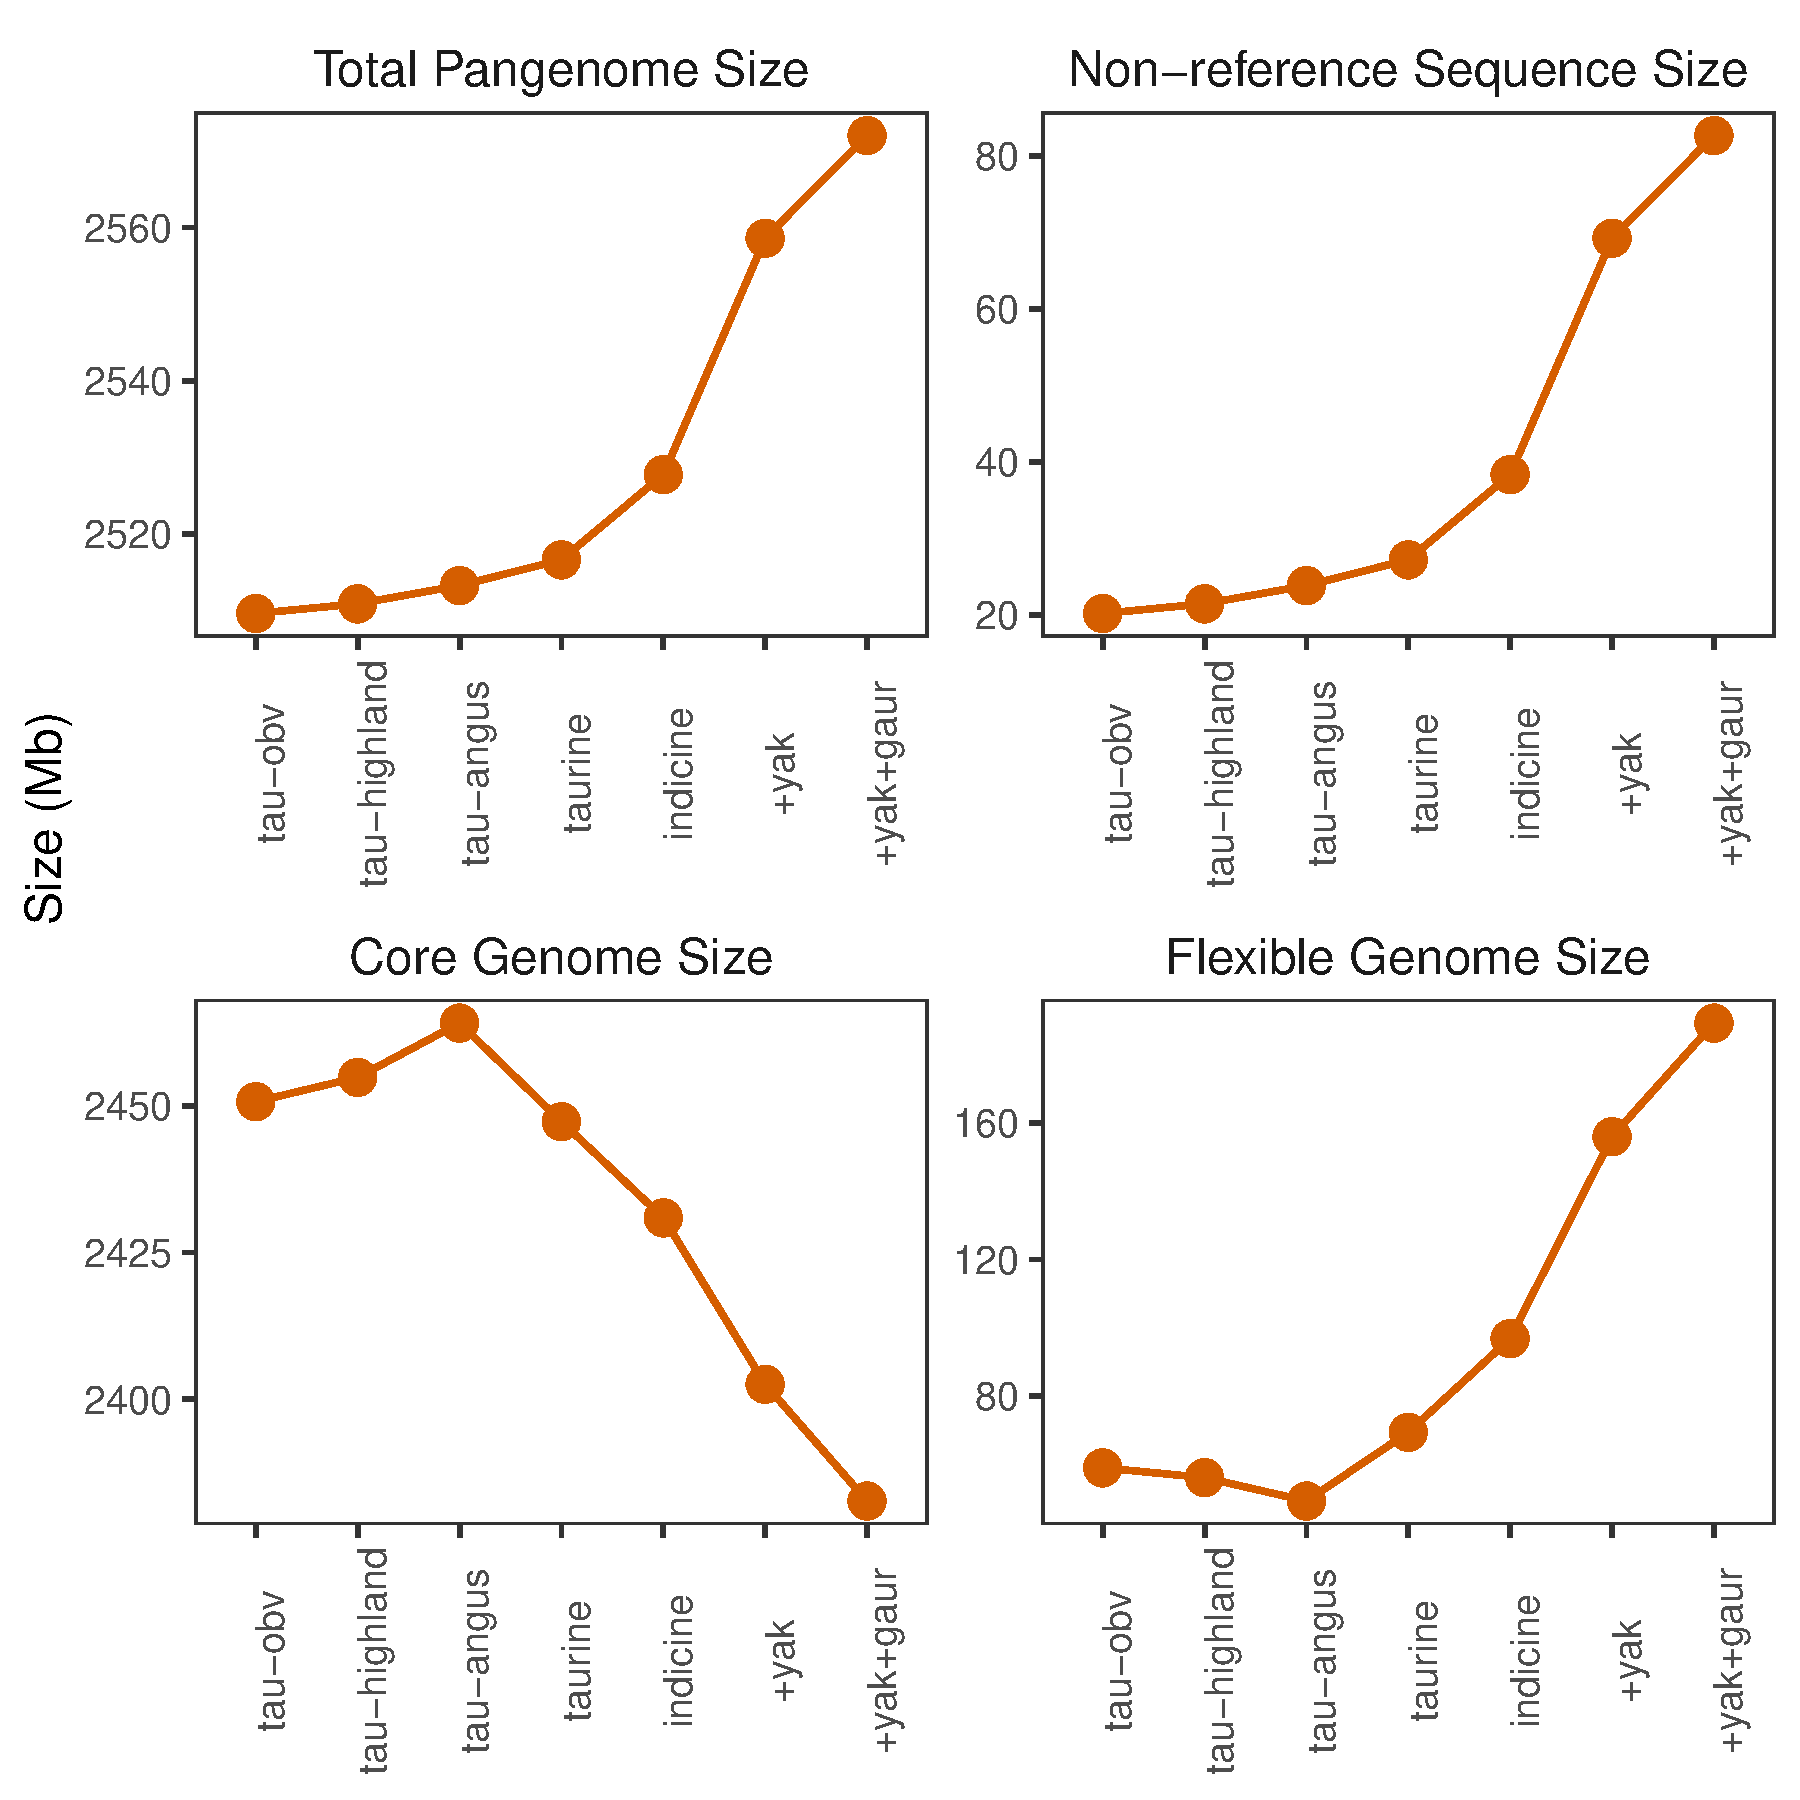
\includegraphics[width=0.9\textwidth]{discuss/fig51.pdf}
       \vspace{3mm}
       \caption[Profile of the pangenome graph]{\textbf{Profile of the pangenome graph} \\
       \footnotesize{Pangenome graphs were constructed as in Chapter 4 (4 taurine breeds, 1 indicine breed, 1 yak) and complemented with a recently available gaur assembly. tau-$X$ denotes a graph with taurine assemblies but excluding breed $X$. Taurine indicates a graph with four taurine breeds. TauInd is a graph consisting of taurine + brahman genomes. +yak and +yak+gaur indicate the TauInd graph with an addition of yak and yak and gaur assembly, respectively. The core and flexible genomes indicate sequences in pangenome shared in all and not in all breeds, respectively.
       }}
       \label{fig51:panchang}
\end{figure}


The construction of a comprehensive pangenome representing global cattle diversity is the major aim of the Bovine Pangenome Consortium \citep{Smith2020}. Chapter 4 provides an initial framework to build such a novel reference structure. A multi-assembly graph built from representative DNA sequences of different cattle breeds might also be a starting point for the construction of a comprehensive bovine pangenome graph that accommodates the full spectrum of genetic variation. The sample selection should be carefully considered to maximize diversity (e.g., some proposed methods \citep{Ros-Freixedes2017,ranallo2021optimized}). The optimal sample selection that includes comprehensive and diverse breeds, including under-represented and wild and undomesticated relatives of cattle, helps to characterize the pangenome of Bovinae that will reveal the true extent of genetic diversity. Since generating reference-quality genome assemblies at the population scale is still cost-prohibitive, an initial assembly-based strategy might be followed by augmenting the multi-assembly graph with known small variations. While small variations can be obtained readily from public databases, Chapter 3 showed that this step is ideally done by iterative augmentation of variations discovered directly from the graphs. Moreover, it seems important to integrate haplotype information in order to indicate biologically plausible allele combinations. The recent development of the so-called dynamic genome graph is appealing as it can be iteratively updated once additional genomes become available and be subdivided into smaller graphs facilitating detailed inspection on the population of interest \citep{eizenga2020efficient}.


\subsection*{Towards establishing highly informative graph genomes that integrate functional genomics resources}

In addition to be comprehensive, graph genomes should be at least as informative as the reference sequence. In their current implementation, graph genomes appear as static entities containing only DNA sequence information. However, the non-linear structure opens the possibility to include additional information in the graph other than DNA sequences, such as allele frequency, phenotype status of individuals (assigned to haplotypes traversing the nodes), or different layers of functional epigenomic data. As a proof of concept, an analysis presented in Chapter 4 showed that labelling the nodes to track sample information enables characterization the origin of the non-reference sequences. For this purpose, a strategy is needed that can compactly store metadata information from large number of samples in the graphs e.g. \citet{siren2020haplotype}. 


Recent studies have examined the possibility of building pangenome graphs that contain information beyond DNA sequences. \citet{Sibbesen2021} showed that adding splice information into a pangenome graph may outperform state-of-the-art RNA sequencing alignment and variant genotyping from linear reference genomes for the analysis of allele-specific expression. \citet{Hokin2020} added genotype information and assigned the disease status of samples, enabling an association study directly from genotype graphs (termed as \emph{Pangenome Wide Association Study}). They found regions harboring complex variations that are associated with complex traits that were missed by traditional GWAS that rely on variants called from linear alignments. On the same line, \citet{kaye2021genome} proposed a Genome Atlas as an informative pangenome representation in which the graph’s nodes are labelled with an unique ID that assigned functional metadata. The connections between nodes are not limited by sequence proximity, e.g. nodes could also be linked because of sharing annotation, which can be flexibly tuned. 

In such an implementation, the pangenome graph can be used as a reference structure for multiple layers of epi-genomics data. This approach is readily feasible in many livestock species for which large amounts of functional omics data have been generated \citep{clark2020faang}. Overall, these graph resources will be highly valuable for the livestock genomics community to catalogue the global livestock diversity in order to perform comprehensive comparative genomics or even to identify beneficial alleles that are relevant for adaptation to future environmental changes.  

\section{Challenges to construct comprehensive pangenome graphs}

\subsection*{Impact of the genome assembly quality on the reliability of the graph-based analysis}

The quality of the assemblies being integrated into the graphs is important. Chapter 2 showed that in regions with unresolved segmental duplications, the graph computation time increased substantially, indicating that the incomplete or flawed assembly of such regions increases graph complexity. Particularly, with the \emph{minigraph} approach, one assembly is used as the backbone of the graph and the pangenome is iteratively built by augmenting other genomes to this backbone. Therefore, the quality of the backbone assembly is critical for accurate and complete pangenome representation, especially to retrieve the true sequences diverged across animals rather than technical artifacts due to the incomplete assembly. Chapter 4 and Fig. \ref{fig52:backeff}  demonstrated that the use of the Highland or OBV assembly as a backbone leads to a larger pangenome and less non-reference sequences detected from the other assemblies. This finding possibly suggests that these two assemblies are more complete than other assemblies which seems to corroborate findings from the initial analysis of the Highland assembly \citep{rice2020continuous}. 

\begin{figure}[!htb]
   \centering
   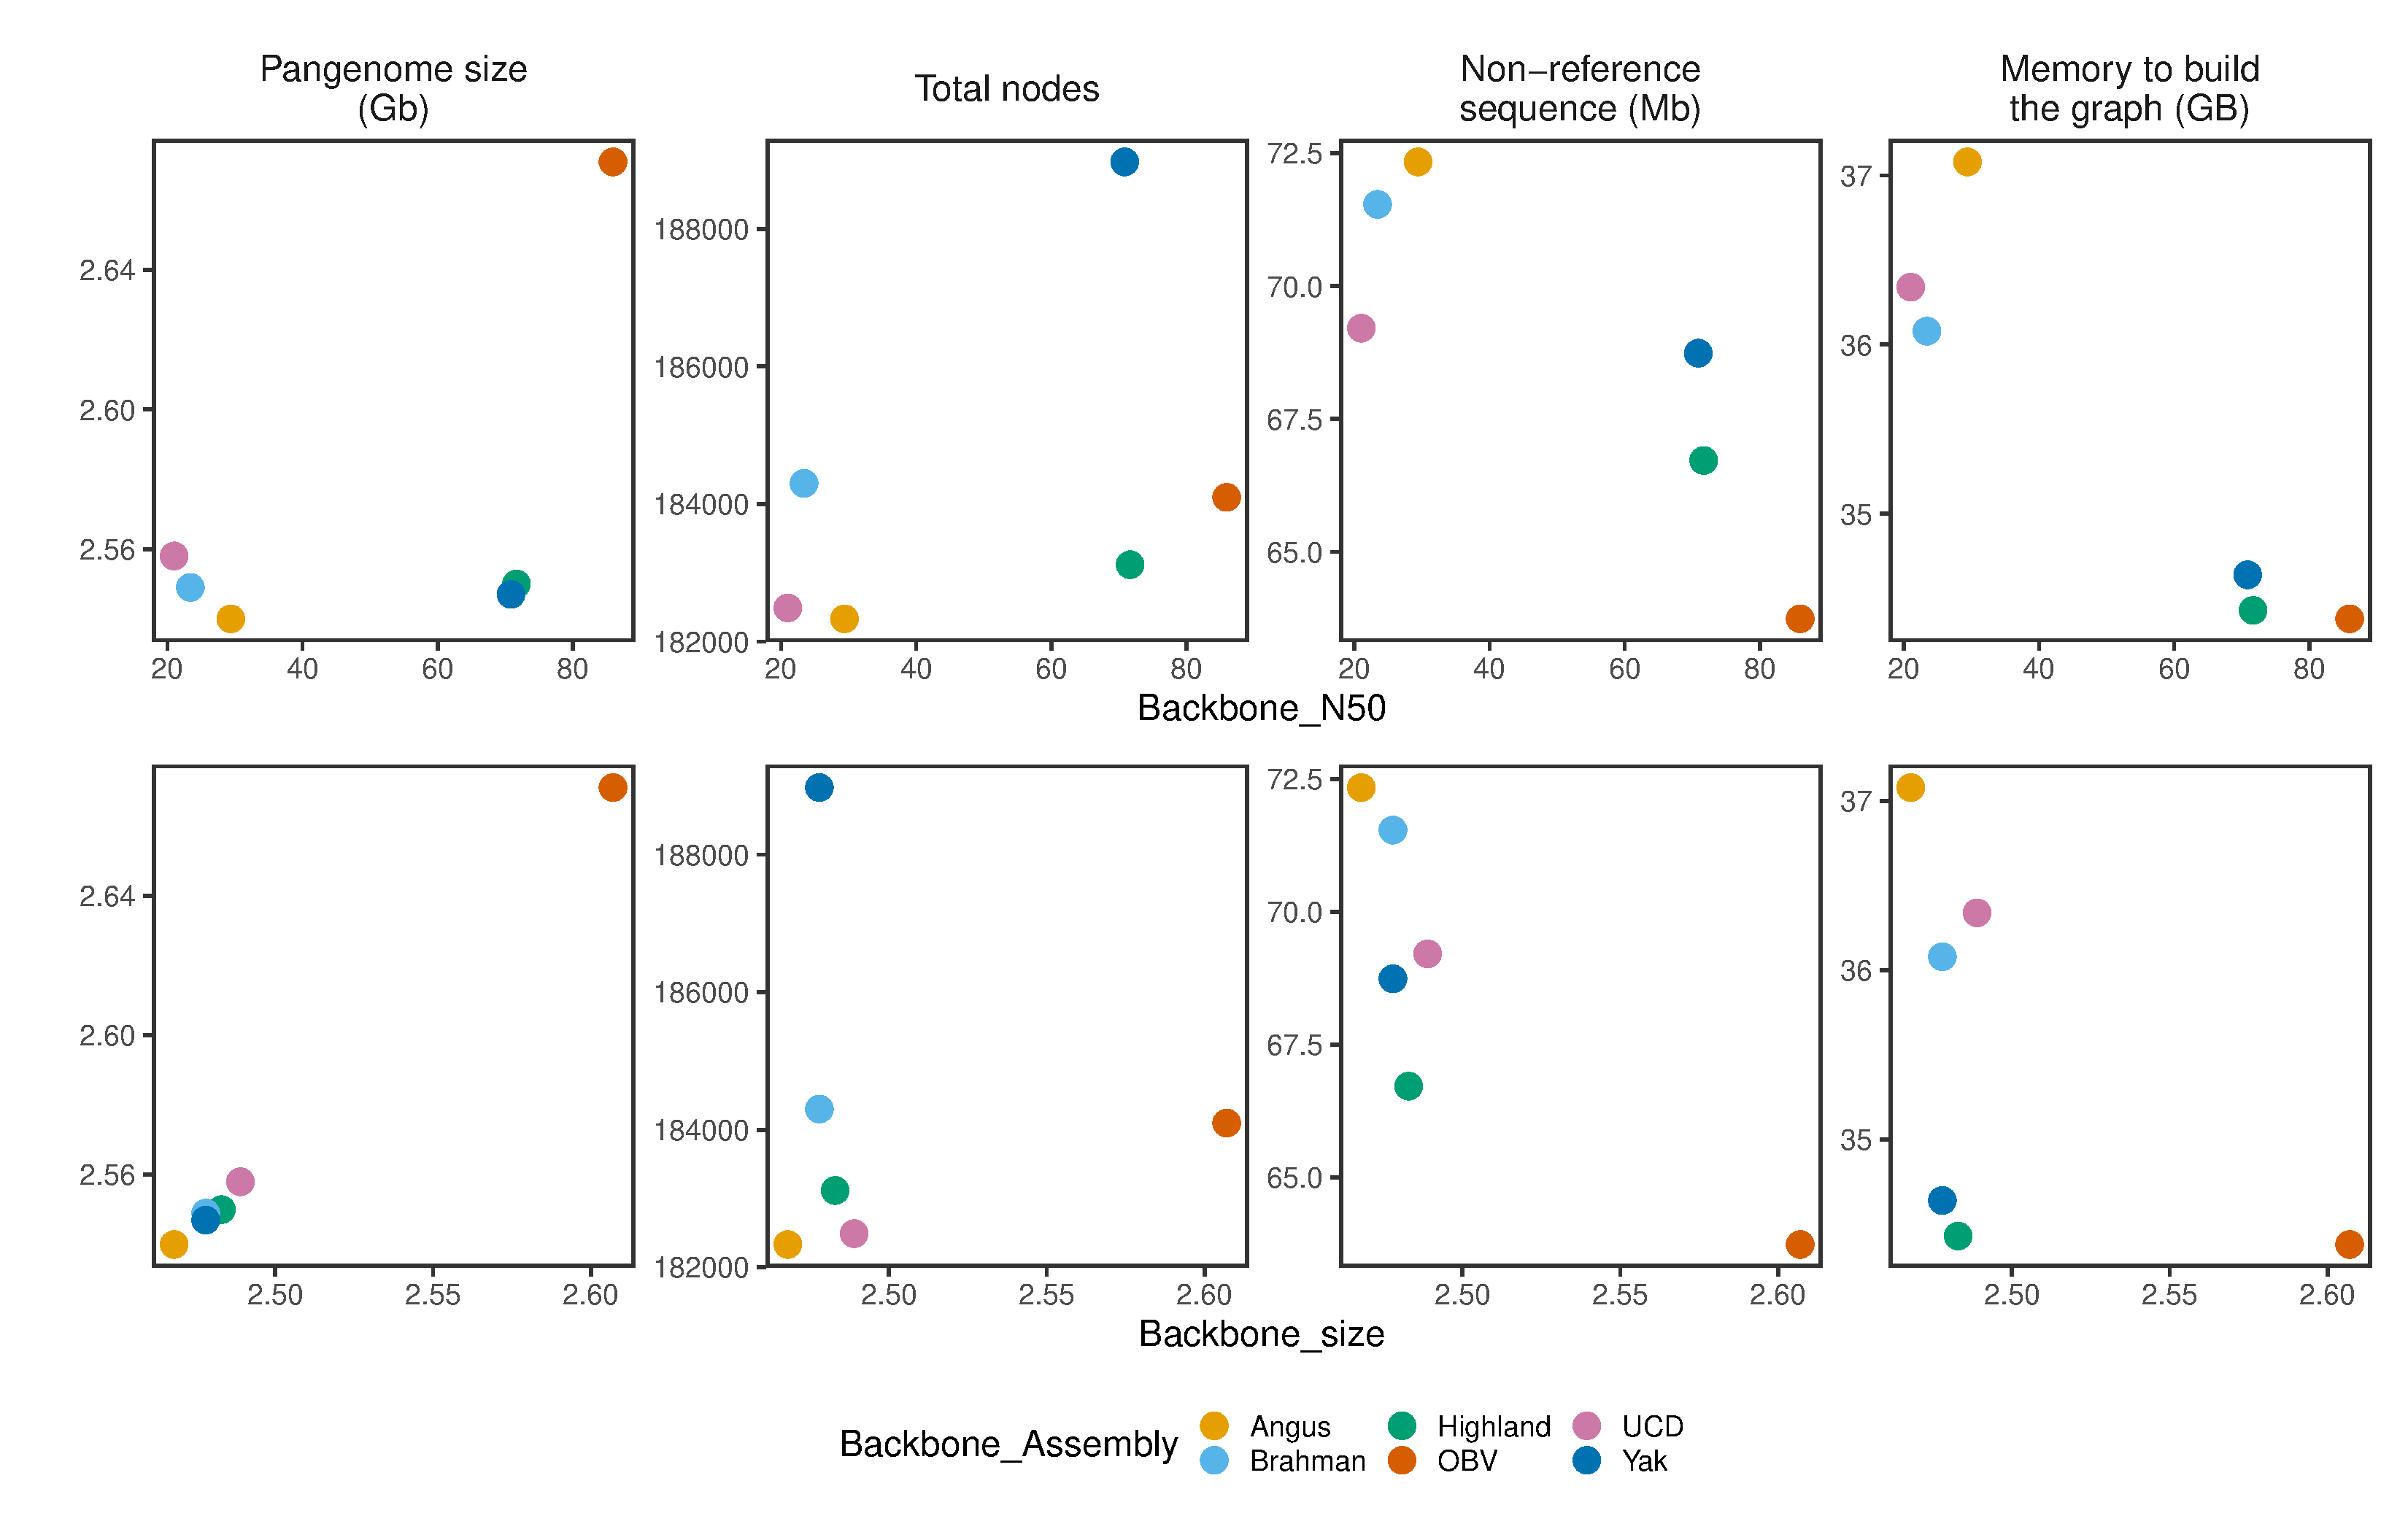
\includegraphics[width=\textwidth]{discuss/fig52.pdf}
       \vspace{1mm}
       \caption[Correlation between the backbone assembly quality and the profile of the pangenome graph]{\textbf{Correlation between the backbone assembly quality and the profile of the pangenome graph} \\
       \footnotesize{A colored dot represents the backbone assembly from which that the graph was built from. 
        N50 represents the assembly contiguity with a higher number reflects a more contiguous assembly. 
       }}
       \label{fig52:backeff}
\end{figure}

Additionally, the pangenome will benefit from the use of haplotype-resolved assemblies. The mapping algorithm in \emph{vg} (Chapter 3) utilizes phasing information to prioritize read alignments conforming to biologically plausible  haplotypes, thus reducing mapping ambiguity. Moreover, haplotype switches in collapsed assemblies might limit the interpretation of long-range information encoded in the paths. The benefit of using haplotype-resolved over primary assemblies has recently been shown in human pangenome, that phasing information helps to infer the genotypes of low-coverage regions facilitating imputation-like strategies performed directly from the graphs \citep{ebler2020pangenome,ebert2021haplotype}. 

Technological advancements in long-read sequencing particularly with the development of the highly-accurate circular consensus sequencing \citep{Wenger2019} facilitate the cost-effective production of high-quality genome assemblies. The multi-assembly graph constructed in Chapter 4 integrated a bovine genome assembly that was generated using HiFi reads. There were 104-116 Mb sequences from the HiFi-based Original Braunvieh assembly not included in the graphs when other assemblies were the backbone of the multi-assembly graph. These sequences are primarily composed of DNA satellites, suggesting that HiFi-reads enable a better assembly of so far difficult-to-assemble regions in the cattle genome, such as telomeric and centromeric sequences. Due to lower quality of X, Y chromosomes, and unplaced contigs, the analyses in this thesis were restricted to the autosomes. The high quality of the novel HiFi-based assemblies now provides an opportunity to also investigate highly polymorphic or repeat regions and sex chromosomes \citep{logsdon2021structure,miga2020telomere}, thus revealing a more accurate and complete pangenome.  

\subsection*{Scalable approaches for building comprehensive pangenome graphs across hundreds of assemblies}

Beyond generating assemblies, scalable approaches that can efficiently construct and characterize a pangenome from many assemblies are needed. The pangenome graph in Chapter 4 was built computationally efficient using the \emph{minigraph}. However, it is unable to represent the full spectrum of genomic diversity as it included only structural variations longer than 50 bp (Table \ref{tab52:mtc}). Thus, to exploit the full potential of the pangenome, full graph models that can accommodate all haplotypes of the individuals in the population and their sites of variations, are required. The development a more comprehensive genome graph such as \emph{pggb} (\url{https://github.com/pangenome/pggb}) or \emph{cactus} \citep{armstrong2020progressive} is promising, because these tools can perform reference-free multi-genome alignment to generate a full graph containing both short and long variations. Utilizing a full pangenome graph as implemented in \emph{pggb} or \emph{cactus} may uncover more variable and non-reference sequences than \emph{minigraph}, as an initial analysis revealed (Table \ref{tab52:mtc}). However, this approach is computationally demanding for whole-genome applications, likely because the resulting graph is more complex due to many small nodes (Table \ref{tab52:mtc}). Additionally, without anchoring the pangenome on well-established reference coordinates, complex and highly repetitive genomic regions tend to form highly tangled regions in the graphs which are difficult to interpret \citep{lei2021plant}. Therefore, a thorough analysis to assess differences between various multi-assembly graph implementations is required. A strategy proposed by the Human Pangenome Reference Consortium to integrate 350 diverse human assemblies is supposed to define the first \emph{de facto} standard in the field. 
\vspace{1em}
\begin{table}[!htb]
   \begin{center}
   \small
   \caption[Comparison of methods to build the multi-assembly graphs]{\textbf{Comparison of methods to build the multi-assembly graphs.} \\
   \footnotesize{Ref nodes refer to the node contained sequences from the ARS-UCD1.2 reference genome and non-ref nodes contained sequences from the other breeds but not in the reference assembly. Core nodes and flexible represent nodes with sequences shared in all breeds and not in all breeds, respectively. R-R, R-NR, NR-NR denote edges connecting ref-ref nodes, ref-non-ref nodes, and non-ref-non-ref nodes respectively.}}
   \vspace{1em}
   \begin{tabular}{|l|l|l|l|l|} 
   \hline
   \multicolumn{1}{|c|}{\textbf{Parameter}} & \multicolumn{1}{c|}{\textbf{Unit}} & \multicolumn{1}{c|}{\textbf{Minigraph pipeline}} & \multicolumn{1}{c|}{\textbf{pggb pipeline}} & \multicolumn{1}{c|}{\textbf{Cactus pipeline}}  \\ 
   \hline
   Average memory                            & Gb                                & 1.7                                            & 12.5                                     & 11.6                                         \\ 
   \hline
   CPU time                                   & hours                           & 0.05                                           & 7.23                                      & 10.98                                         \\ 
   \hline
   All nodes                                 & n                                  & 1,136                                            & 804,723                                     & 843,177                                        \\ 
   \hline
   Total length                              & bp                                 & 42,671,567                                       & 43,495,189                                  & 43,583,632                                     \\ 
   \hline
   Average Node length                       & bp                                 & 37562                                            & 54                                          & 51                                             \\ 
   \hline
   Reference nodes                           & n                                  & 770                                              & 534,993                                     & 545,952                                        \\ 
   \hline
   Total length ref nodes                    & bp                                 & 42,350,435                                       & 42,316,615                                  & 42,350,435                                     \\ 
   \hline
   Non-reference nodes                       & n                                  & 366                                              & 269,730                                     & 297,225                                        \\ 
   \hline
   Total length non-ref nodes                & bp                                 & 321,132                                          & 1,178,574                                   & 1,233,197                                      \\ 
   \hline
   Total edges                               & n                                  & 1,630                                            & 1,384,318                                   & 1,142,667                                      \\ 
   \hline
   R-R edges                                 & n                                  & 904                                              & 706,505                                     & 570,277                                        \\ 
   \hline
   R-NR edges                                & n                                  & 705                                              & 631,949                                     & 524,483                                        \\ 
   \hline
   NR-NR edges                               & n                                  & 21                                               & 45,864                                      & 47,907                                         \\ 
   \hline
   Node to Edge Ratio                        & ratio                              & 1.43                                             & 1.72                                        & 1.35                                           \\ 
   \hline
   Core nodes                                & n                                  & 441                                              & 270,044                                     & 274,134                                        \\ 
   \hline
   Core length                               & bp                                 & 42,071,986                                       & 41,546,904                                  & 41,577,514                                     \\ 
   \hline
   Flexible nodes                            & n                                  & 695                                              & 534,679                                     & 569,043                                        \\ 
   \hline
   Flexible length                           & bp                                 & 59,9581                                          & 1,948,285                                   & 2,006,118                                      \\ 
   \hline
   Core proportion                           & \%                                 & 98.59\%                                          & 95.52\%                                     & 95.39\%                                        \\ 
   \hline
   Flexible proportion                       & \%                                 & 1.41\%                                           & 4.48\%                                      & 4.60\%                                         \\
   \hline
   \end{tabular}
   \label{tab52:mtc}
   \end{center}
   \footnotesize{$^*$ The multi-assembly graph was built from chromosome 25 of 4 taurine assemblies (Hereford, Angus, Highland, Original Braunvieh) and 1 indicine (Brahman) assembly. The minigraph pipeline was implemented as in the Chapter 4. The pggb pipeline was run with the recommended parameters (\texttt{-s 100000 -p 90 -n 10}, \url{https://github.com/pangenome/pggb}) and the cactus pipeline was based on the suggested within-species pangenome pipeline (\url{https://github.com/ComparativeGenomicsToolkit/cactus}). Both pggb and cactus pipeline implement a full graph model that includes complete variations, meanwhile minigraph only considers variations longer than 50 bp. \\
   }
\end{table}

\subsection*{Stable ecosystem of tools and adoption of graph genomes in the genomics community}

A stable framework to efficiently store, modify, and handle complex graphs for routine genomic analyses remains to be developed. Many analyses presented in this thesis were not fully graph-based as they depend on the graph’s transformation into linear coordinates to make the graph amenable to current tools. For example, sequence variant genotyping in Chapter 3 was based on projections onto reference sequence paths. Thus, the reported improvement of genotyping accuracy over linear alignments might be more pronounced once all analyses are performed directly on the graph. Moreover, multiple fragmented graph implementations for specific use cases with poor interoperability among the tools hamper the development of widely-accepted graph-based genomics approaches. For example, due to different specifications, the graph structure from \emph{minigraph} (Chapter 4) is not compatible with extensive graph operations that have been implemented in \emph{vg} (Chapter 3). As the graph genome framework reaches maturity, the genomics community ideally will agree on a widely-accepted standard that ensures long-term stability, similar to  tools development for the linear reference genome (e.g., \emph{BAM}, \emph{VCF}) \citep{bonfield2021htslib}. A wider adoption of graph-based analysis will naturally foster the development of efficient tools to process these new richer reference structures (e.g., \citep{qiu2021constructing,schulz2020detecting}).

Reluctance of the genomics community to transition to graph-based approaches results in slower adoption of the methods. It is clear that a transition to a graph-based reference will require a new paradigm and huge efforts to adjust downstream tools that rely on a linear representation of the genome. Additionally, instead of a ready-to-use linear genome, graph genomes need a more involved construction process (see Chapter 3 Methods). However, this thesis clearly showed that the increase in the analysis complexity is outweighed by novel intriguing insights. Moreover, graph-based structures are required to compactly integrate an ever-increasing amount of genomic resources. To increase the appeal of graph-based genomes, it is highly desirable to have a robust graph-genome-based visualization for interactive explorations of the graph structure (e.g. coloring paths according to breeds that might help pinpoint segments differentiating between lineages). However, implementations that can accommodate across zoom levels and finer details are still not fully operable \citep{yokoyama2019momi,beyer2019sequence,eizenga2020pangenome}. In the short term, graph-based approaches may be used for intermediate steps which are hidden from the end user, i.e., the analysis is performed on graphs but the output is projected back to the linear space. Thus, graphs might supplement rather than completely replace linear genomes \citep{kim2019graph,grytten2020assessing,li2020design,siren2020genotyping}. The \emph{Graphtyper} pipeline as implemented in Chapter 2 follows this paradigm. 

\newpage

\fancyhead[C]{OUTLOOK}
\section*{\LARGE{Outlook}}
\phantomsection
\addcontentsline{toc}{chapter}{Outlook}
\thispagestyle{plain}

This thesis presents the first implementations of graph-based reference structures in cattle. Pangenome graphs provide a framework for accurate, unbiased and complete representation of sequence variation within a species, including those that are missed in routine genomic analysis because of the incompleteness of a single linear reference genome. The graph-based approaches presented in this thesis may serve as a starting point for many analyses that have either not yet been possible or were less accurate due to using the linear reference sequence. Importantly, this thesis provides a computational framework to integrate and exploit an ever-increasing amount of genomic resources (including genome assemblies and their sites of variation). On the one hand, this is relevant for collaborative initiatives to catalogue the complete species diversity such as the Bovine Pangenome Consortium. On the other hand, the computational framework developed and implemented in this thesis is broadly applicable to many species. Importantly, comprehensive comparative genomic analyses on the pangenome graph might help identify genomic features that are conserved or diverged between breeds and species that might underly the adaptive traits or domestication which can then be exploited to accelerate genetic progress \citep{foissac2019multi,clark2020faang}. 

Potential applications of genome graphs to enhance livestock genomics are discussed below

\subsection*{Unbiased genomic analyses using genome graphs}

Genome graph approaches provide an opportunity to revisit genomic analyses that suffer from reference bias, such as allele-specific expression (ASE), which attempts to detect gene expression imbalance between paternal and maternal-derived alleles \citep{castel2020vast}. ASE is known to be pervasive in the cattle genome \citep{chamberlain2015extensive} and affects complex traits in livestock such as meat quality \citep{guillocheau2019survey,bruscadin2021muscle}. The current ASE detection method primarily relies on RNA-sequencing alignments to a linear genome which is prone to reference allele bias. To overcome this issue, reference sequences are commonly modified to match the alleles from the transcriptome \citep{salavati2019elimination}. However, this strategy is imperfect as it needs two rounds of read mapping, is limited to SNPs, and can still underestimate the overall expression levels \citep{van2015wasp}. Genome graphs can represent both paternal and maternal alleles in a coherent structure that can mitigate this issue. The split-read mapping capability that has been recently implemented in the \emph{vg toolkit} \citep{Sibbesen2021} facilitates direct mapping of transcriptome data against genome graphs. Therefore, it is appealing to perform a more accurate ASE analysis in livestock using the graph genome approach. 

\subsection*{Comprehensive variations from pangenome might contribute to the missing heritability and improve genomic predictions}

Even the most comprehensive catalogues of genetic variations available to date cannot capture the full heritability of traits, widely known as missing heritability \citep{maher2008personal}. For example, a large meta-analysis on stature in cattle identified 163 lead variants, but these variants only explain about 13.8\% of the heritability of stature \citep{bouwman2018meta}. There were some proposals explaining the sources of missing heritability, such as the contribution of rarer variants \citep{gonzalez2015rare} that can be recovered when considering large mapping cohorts that have been genotyped directly for whole-genome variations \citep{wainschtein2019recovery}. However, complex structural variations and sequences not present in the reference genome which are not routinely assessed might as well contribute to the missing heritability \citep{genin2020missing,theunissen2020structural}. The effect of large variations can be completely missed, which undermine its contribution to the genetic of traits. 

Several studies in humans \citep{eggertsson2019graphtyper2,chen2019paragraph,hickey2020genotyping} have attempted to integrate sequence-resolved large structural variations that were detected using long read sequencing into pangenome graphs. These variations may then serve as a reference for reference-guided variant discovery from short-read sequencing data. The graph-based structures developed in this thesis provide an appealing resource to call genotypes at large structural variants from the vast amount of whole-genome short-read re-sequencing data that have been collected in many breeds of cattle. These genotypes may then  be used for robust genetic studies that might uncover some part of the missing heritability.

Genotypes at genome-wide variants are frequently used to predict the animal’s genetic merit, widely known as genomic prediction \citep{meuwissen2001prediction}. Genomic prediction typically relies on SNPs and small insertion and deletion polymorphisms detected from a linear reference genome. Recent efforts aimed at including genotypes from structural variations in the genomic prediction models. However, these structural variations only resulted in small improvements in prediction accuracy over pure SNP-based prediction \citep{el2018genomic,chen2021investigating}. This might be partly due to an incomplete representation of structural variations from short-read sequencing data aligned to linear coordinates. Pangenome graphs offer the ability to catalogue more accurate and unbiased variations from the population, particularly at genomic regions that are missing in the reference genome. These hitherto neglected variants may improve the prediction accuracy, thus leading to additional genetic gain. Additionally, informative graph genomes that integrate diverse functional omics data might be used to prioritize variants in genomic prediction. \citet{macleod2016exploiting} showed that stratification of variants with functional omics data improves prediction accuracy over treating all variants equally. 


\subsection*{Sequence variants in the pangenome might be causative for agriculturally important traits}

Most of the genomic analyses in livestock rely on genetic markers discovered from a linear reference genome. Thus, association testing between phenotypes and markers is blind to variants in segments that are missing in the linear reference sequence. Several studies in plants and humans have shown that important QTL may be missed in genomic regions that are absent from the reference \citep{kehr2017diversity,gage2019multiple,song2020eight}. Additionally, the fine mapping of causative variants is challenging in genomic regions harboring structural variants that are not part of the reference sequences. On the other hand, the contribution of large variations to the genetic architecture of complex traits may be substantial. \citet{chiang2017impact} and \citet{chaisson2019multi} suggest that large structural variations are more likely to be associated with GWAS signals due to having larger impacts on gene expression than SNPs. \citet{song2020eight} performed GWAS between phenotypes and presence-absence variations of pangenome segments (termed as PAV GWAS) across \emph{Brassica} accessions  to identify large insertions, not part of the reference sequences, as causal variants for agriculturally important traits. Moreover, a pangenome-based analysis of more than 15,000 Icelandic genomes uncovered a common 766 bp insertion \citep{kehr2017diversity} that is associated with a complex trait. These series of studies highlight interesting areas for potential applications of pangenome-based analyses to dissect the genetic architecture of complex traits, which have not been applied to livestock populations. \citet{hayes20191000} noted that the rate of causal variant identification for complex traits has been very slow in cattle, which might partially be due to not considering many variants that are not accessible from the existing linear reference genome. 

\subsection*{Resources to catalogue and preserve the complete genetic diversity}

Domestication and selection of livestock species resulted in a considerable reduction of the genetic diversity compared to the wild relatives (termed as \emph{the cost of domestication}) \citep{mchugo2019unlocking}. Selection for desirable genes might be accompanied by unintentional removal of beneficial variants related to disease-, parasite-  or heat resilience relevant to potentially changing environmental conditions. Thus, the cosmopolitan breeds might be more susceptible to environmental stress. For example, breeding for milk yield in dairy cattle is accompanied with undesired impacts on fertility \citep{pryce2004fertility} and there is a negative genetic correlation between milk yield and mastitis resistance \citep{cai2020distinguishing}. 

Targeting non-domesticated relatives in the pangenome might help to identify genetic diversity which has been lost due to domestication and breeding that might be favorable for the future environmental changes \citep{khan2020super}. Such a \emph{super pangenome} of extant and extinct relatives of domestic species might uncover alleles that were lost during domestication that can be re-introgressed into the modern breeds. Of note, genome assemblies of undomesticated Bovinae members of bison (\emph{Bison bison}) \citep{oppenheimer2021reference} and gaur (\emph{Bos gaurus}) have been created recently, providing an opportunity to enrich the bovine pangenome with more diversity (Fig. \ref{fig51:panchang}). Additionally, the trio binning assembly technique performs better for trios with diverged parents \citep{rice2020continuous,heaton2021reference}. This provides exciting opportunities to generate assemblies for understudied or undomesticated cattle relatives that will generate diverse collections cattle assemblies that become ideal resources to construct a comprehensive bovine pangenome.

\fancyhead[C]{REFERENCES}
\singlespacing
\footnotesize

% uncomment so that references appear on the same page
% \let\Origclearpage\clearpage
% \let\clearpage\relax

\bibliographystyle{unsrtnat}
\bibliography{references/discuss_ref}
%\printbibliography[title=References]

% \let\clearpage\Origclearpage

\ifdefined\BuildingFromMainFile
\else
   \end{document}
\fi